\section{Umsetzung virtueller Spiele in der physischen Welt}

Unter einem virtuellen Spiel verstehen wir jene, die sich ausschlie�lich  auf einem Computer spielen lassen.
Es folgen eine Reihe virtueller Spiele, die sich f�r die Integration in die physische Welt eignen.
\subsection*{Snake}
Ein absoluter Klassiker, der fr�her auf keinem Handy fehlen durfte. 
%Gerade wegen der Popularit�t und Einfachheit recht interessant es in die physische Welt zu integrieren. 
In einem begrenzten Areal gilt es eine Schlange geschickt zu steuern. Es m�ssen Items eingesammelt werden, wodurch die Schlange w�chst. Au�erdem muss darauf geachtet werden, dass weder der Rand des Areals noch die eigene Schlange ber�hrt wird.


\begin{figure}[htbp]
  \centering
    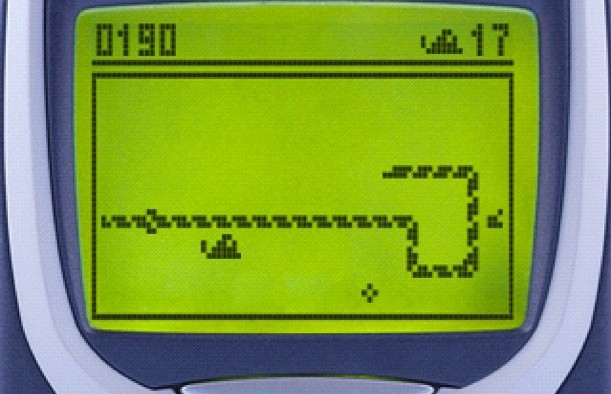
\includegraphics[width=0.5\textwidth]{2-Spielideen/2-1-Umsetzung_virtueller_Spiele_in_der_physischen_Welt/snake.png}
     \caption{Snake auf dem Nokia 3310 
		(Quelle: \url{http://nixtv.de/wp-content/uploads/2014/09/snake.jpg}) }
\end{figure}

Snake ist vielen nur als Einzelspieler-Spiel bekannt. Da wir es als Outdoor-Bewegungsspiel umsetzen und es un�blich ist diese alleine allein zu spielen, haben wir entschieden, Snake in der physischen Welt als Mehrspieler-Spiel umzusetzen, in dem wir als Spielfeld eine reelle Karte nehmen.  Wie wir dies umgesetzt haben, wird sp�ter erl�utert.

\subsection*{Capture the Flag}
Das Spiel ist nicht nur als virtuelles Spiel geeignet, wurde als solches aber erst richtig bekannt. Der relativ einfacher Spielmechanismus erleichtert den  Einsatz in der physischen Welt. Zwei Teams treten gegeneinander an. Jedes Team besitzt eine Basis mit einer Flagge, dessen Standort f�r das gegnerische Team bekannt ist. Es wird versucht die Flagge des jeweils anderen Teams zur eigenen Basis zu bringen. Gelingt dies w�hrend die eigene Flagge nicht vom gegnerischen Team "`entf�hrt"' wurde, erh�lt das eigene Team Punkte. Wird eine gewisse Punktzahl erreicht, gilt das Spiel als gewonnen.

Problematisch im Falle einer Umsetzung ist, dass man in der Regel gegnerische Spieler "ausschalten" kann und diese dann in die eigene Basis zur�ckgesetzt werden. Dies muss im Fall einer Umsetzung anders realisiert werden.

Hilfreich bei der Integration in die physische Welt w�ren zum einen eine Richtungsangabe der Basis des gegnerischen Teams oder gar eine Karte, auf der die Basis angezeigt wird (eventuell auch die Position der eigenen Flagge, Position der Mitspieler, etc.), zum anderen der aktuelle Punktestand der Teams (eventuell mit Highscore).

\subsection*{Domination}
Meist in Kriegsszenarien integrierter virtueller Spielmodus, der sich mit wenig Aufwand in die physische Welt �bertragen l�sst. Zwei Teams treten gegeneinander an. Jedes Team hat einen Punktestand, der zu Anfang gleich ist, sich aber stetig verringert. Sinkt der Punktestand auf null, so ist das Spiel f�r dieses Team verloren. Es gibt verschiedene Areale, die eingenommen werden k�nnen. Ein Team kann ein Areal einnehmen in dem sich dort f�r einen gewissen Zeitraum mehr eigene Mitglieder als Mitglieder  des gegnerischen Teams befinden. Hierbei ist es m�glich gegnerische Spieler "auszuschalten". Diese starten dann wieder in einer Startzone. Auch hier m�sste dieses Spielelement im Falle einer Umsetzung anders realisiert werden. Hat ein Team mehr Areale eingenommen als das Andere, l�uft der Punktestand des Teams, das weniger Areale in besitzt hat, schneller gegen Null.

Um dieses Spiel in die physische Welt zu integrieren w�re die Anzeige einer Karte wichtig. Auf dieser sollten wichtige Informationen wie z.B. Position der einnehmbaren Areale sein, und wer sie kontrolliert. Eine Anzeige �ber den Punktestand, also Informationen �ber den Verlauf des Spiels w�re ebenfalls wichtig.

 %Verwirklicht werden kann das ganze, indem vor allem der Punktestand umgesetzt wird. Ebenfalls nicht unwichtig ist die Anzeige (z.B. auf einer Karte) der einzunehmenden Areale und in welchem Besitz sie sich gerade befinden. Au�erdem k�nnte dargestellt werden wo sich die eigenen Teammitglieder befinden.